\documentclass[12pt,a4paper]{article}

\usepackage[T2A]{fontenc}
\usepackage[utf8]{inputenc}
\usepackage[russian]{babel}
\usepackage{amsmath,amssymb}
\usepackage{graphicx}
\usepackage{float}
\usepackage{geometry}
\usepackage{caption}
\usepackage{indentfirst}

\geometry{left=25mm,right=20mm,top=20mm,bottom=25mm}
\setlength{\parindent}{1.25cm}
\setlength{\parskip}{0pt}
\numberwithin{equation}{section}
\graphicspath{{images/}}

\newcommand{\documentfigure}[3]{%
\begin{figure}[H]
    \centering
    \includegraphics[#2]{#1}
    \caption{#3}
\end{figure}%
}

\newcommand{\fillValue}[1]{\underline{\hspace{#1}}}

\newcommand{\graphPlaceholder}[2]{%
\begin{figure}[H]
    \centering
    \fbox{\parbox[c][55mm][c]{0.88\textwidth}{\centering
        Место для графика\\[0.5em]
        \textbf{#1}}}
    \caption{#2}
\end{figure}%
}

\begin{document}

\begin{center}
    \textbf{Лабораторная работа 2.1.5}\\[0.8em]
    {\Large \textbf{Исследование термических эффектов\\при упругих деформациях}}
\end{center}

\textbf{Цель работы:} экспериментально получить закон упругой деформации резины при постоянной температуре в зависимости от растягивающей силы; измерить нагрев резины при адиабатическом растяжении и определить её теплоёмкость.

\textbf{В работе используются:} образец резины (тонкая полоса), закреплённый в теплоизолированном кожухе; набор грузов; термопара; цифровой осциллограф или микровольтметр.

Большинство тел при нагреве расширяется, поэтому при адиабатическом растяжении охлаждается. Резина проявляет обратный эффект: под постоянной нагрузкой она при нагреве сжимается, а при адиабатическом растяжении нагревается.

Резина способна многократно удлиняться без разрушения. Её коэффициент Пуассона близок к $\mu \approx 0{,}5$, поэтому объём при растяжении почти не меняется. Деформация происходит главным образом за счёт переориентации звеньев полимерных цепочек, что определяет необычные механические и термические свойства материала.

\section*{Теоретические сведения}

При растяжении полосы длиной $l$ силой $f$ работа образца равна
\begin{equation}\tag{1}
    \delta A = - f\,dl + P\,dV,
\end{equation}
где $P$ --- атмосферное давление. Поскольку изменение объёма мало, слагаемым $P\,dV$ можно пренебречь. Первое начало термодинамики принимает вид
\begin{equation}\tag{2}
    dU \approx T\,dS + f\,dl,
\end{equation}
где $T\,dS = \delta Q$ --- переданная образцу теплота.

\begin{figure}[H]
    \centering
    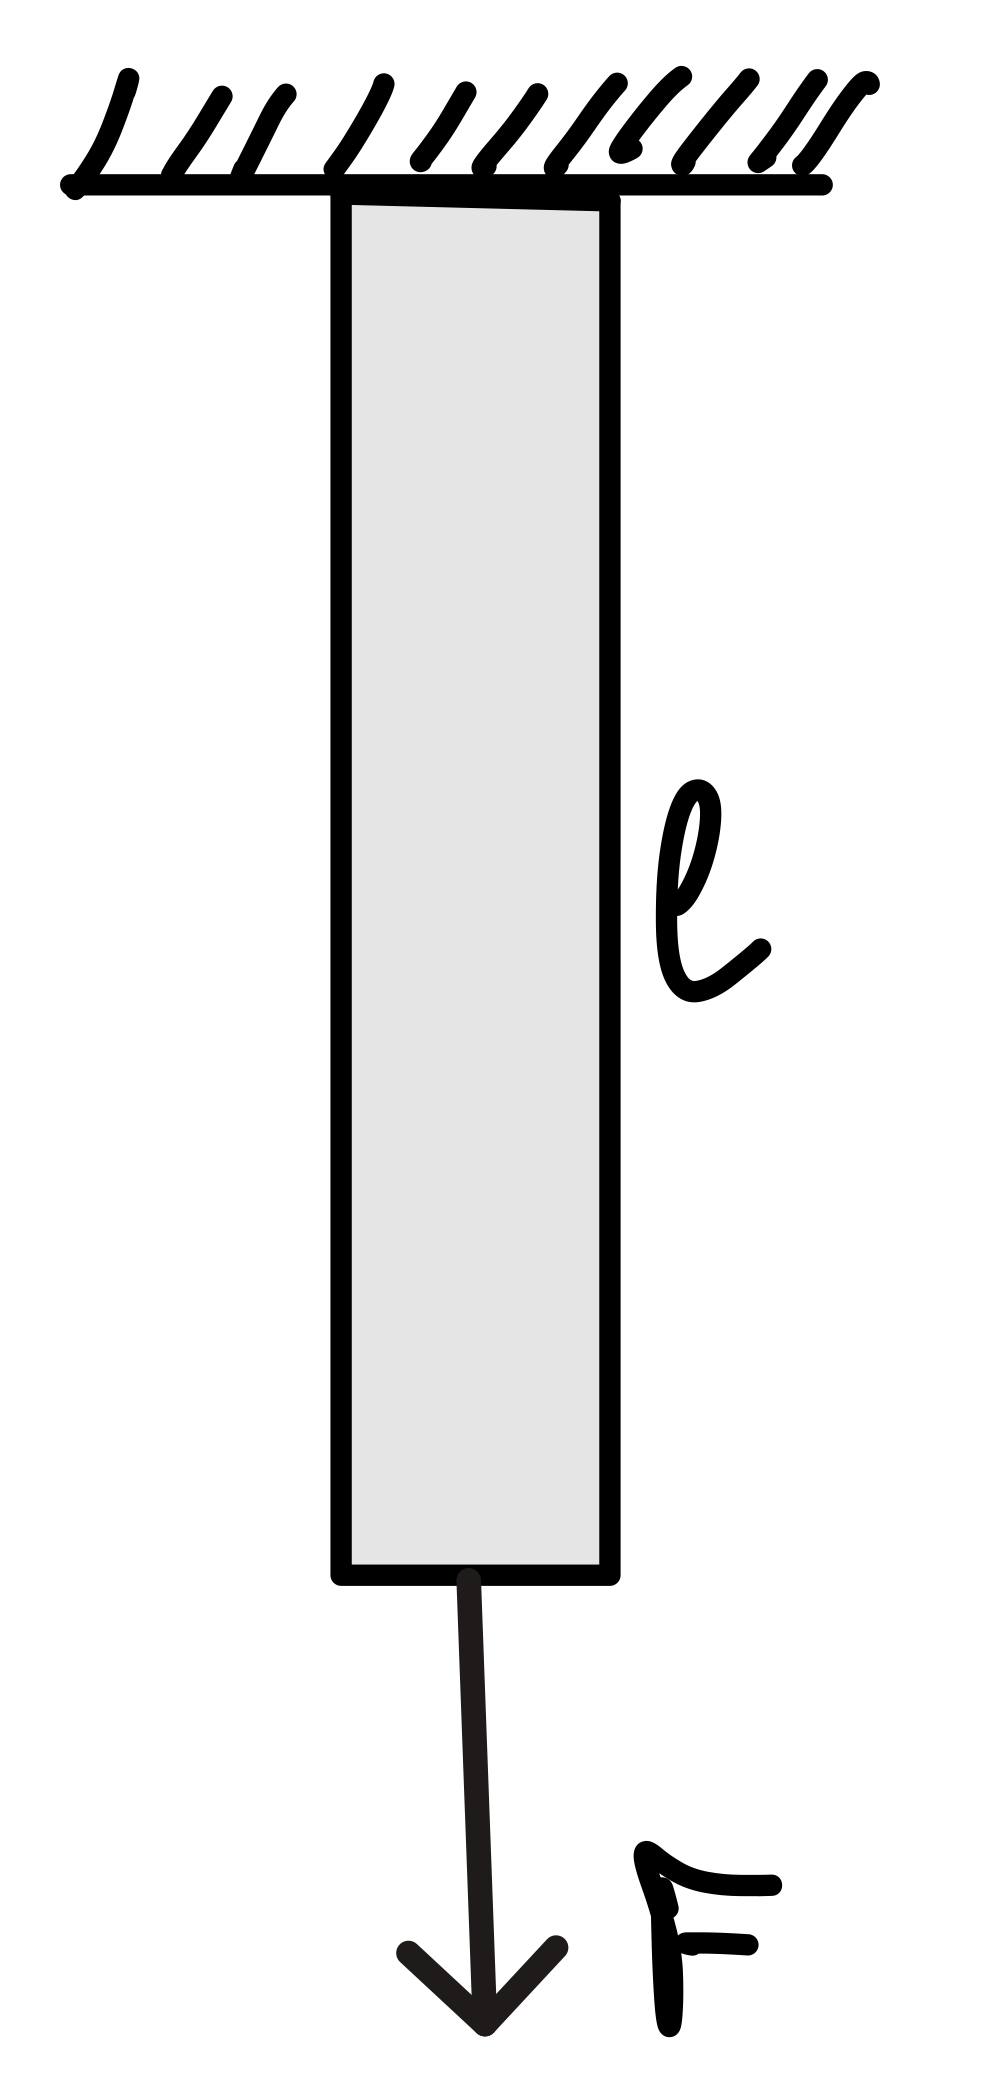
\includegraphics[height=35mm,keepaspectratio]{stretch_scheme.jpeg}
    \caption*{Схема растяжения тонкой полосы или стержня}
\end{figure}

В изотермическом процессе удобно использовать свободную энергию
\begin{equation}\tag{3}
    F = U - TS.
\end{equation}
Её приращение равно работе внешних сил:
\[
    \Delta F\big|_T = \Delta U - T\Delta S = \Delta U - Q = A_{\text{внеш}}.
\]
С учётом (2)
\begin{equation}\tag{4}
    dF = -S\,dT + f\,dl.
\end{equation}
Следовательно,
\begin{equation}\tag{5}
    f = \left(\frac{\partial F}{\partial l}\right)_T, \qquad
    S = -\left(\frac{\partial F}{\partial T}\right)_l.
\end{equation}
Отсюда внутренняя энергия выражается как
\begin{equation}\tag{6}
    U(T,l) = F(T,l) - T\left(\frac{\partial F}{\partial T}\right)_l
\end{equation}
(соотношение Гиббса--Гельмгольца).

Из равенства смешанных производных
\[
    \frac{\partial^2 F}{\partial l\,\partial T}
    =
    \frac{\partial^2 F}{\partial T\,\partial l},
\]
следует соотношение Максвелла
\begin{equation}\tag{7}
    \left(\frac{\partial f}{\partial T}\right)_l
    =
    -\left(\frac{\partial S}{\partial l}\right)_T.
\end{equation}
Отсюда выражение для теплоты изотермического растяжения:
\[
    \delta Q\big|_T = T\,dS\big|_T
    = T\left(\frac{\partial S}{\partial l}\right)_T dl\big|_T
    = -T\left(\frac{\partial f}{\partial T}\right)_l dl\big|_T.
\]

Из первого начала при постоянной температуре получаем связь термического и калорического уравнений состояния:
\begin{equation}\tag{8}
    f = \left(\frac{\partial U}{\partial l}\right)_T
    - T\left(\frac{\partial S}{\partial l}\right)_T.
\end{equation}
В обычных твёрдых телах преобладает энергетическое слагаемое, а в резине --- энтропийное.

\textbf{Термодинамика резины.} В модели идеальной резины внутренняя энергия не зависит от длины:
\begin{equation}\tag{9}
    U = U(T).
\end{equation}
Это приближение применимо, поскольку при почти постоянном объёме средние межмолекулярные расстояния меняются слабо.

При изотермическом растяжении $dU=0$, поэтому
\[
    \delta Q = T\,dS = - f\,dl
    \quad \Rightarrow \quad
    Q = -\int f\,dl = -A_{\text{внеш}}.
\]
Следовательно, при изотермическом растяжении резина выделяет тепло: $Q<0$.

Из (8) при $\left(\partial U/\partial l\right)_T=0$
\begin{equation}\tag{10}
    f = -T\left(\frac{\partial S}{\partial l}\right)_T.
\end{equation}
Следовательно, сила упругости определяется уменьшением энтропии.

Совместно с (7) это даёт
\begin{equation}\tag{11}
    f = T\left(\frac{\partial f}{\partial T}\right)_l.
\end{equation}
Отсюда сила пропорциональна абсолютной температуре:
\begin{equation}\tag{12}
    f(T,l) = \frac{T}{T_0}\,\tilde f\left(\frac{l}{l_0}\right),
\end{equation}
где $\tilde f(l/l_0)$ зависит только от относительного растяжения. Следовательно, модуль Юнга идеальной резины также пропорционален температуре.

При обратимом адиабатическом растяжении $dS=0$, поэтому
\[
    dU = f\,dl.
\]
С другой стороны,
\[
    dU = C_l\,dT,
\]
где $C_l$ --- теплоёмкость при постоянном удлинении. При $\Delta T\ll T$
\begin{equation}\tag{13}
    \Delta T \approx \frac{1}{C_l}\int_{l_0}^{l} f\,dl
    = \frac{A_{\text{внеш}}}{C_l}.
\end{equation}
Таким образом, нагрев пропорционален работе внешних сил.

Из (2) также следует
\[
    dS = C_l\frac{dT}{T} - \frac{f\,dl}{T_0}
\]
откуда
\begin{equation}\tag{14}
    \Delta S = C_l\ln\frac{T}{T_0} - \frac{1}{T_0}\int_{l_0}^{l} f\,dl.
\end{equation}
При растяжении энтропия уменьшается; в изэнтропическом процессе это компенсируется повышением температуры. При $\Delta T\ll T_0$ формула (14) переходит в (13).

\textbf{Закон растяжения резины.} В модели идеальной полимерной сетки при $T=\mathrm{const}$
\begin{equation}\tag{15}
    \Delta S(\lambda) \approx -\mathrm{const}\cdot\left(\lambda^2 + \frac{2}{\lambda}\right),
\end{equation}
где $\lambda=l/l_0$ --- относительное растяжение. Подстановка (15) в (10) даёт
\begin{equation}\tag{16}
    f(T,\lambda) = s_0 E\cdot \frac{1}{3}\left(\lambda - \frac{1}{\lambda^2}\right).
\end{equation}
Здесь $s_0$ --- начальная площадь поперечного сечения, $E=E_0T/T_0$. При $\lambda\to1$ формула переходит в закон Гука $f\approx s_0E(\lambda-1)$.

\textbf{Адиабатическое растяжение в общем случае.} Для произвольного материала справедливо тождество
\[
    \left(\frac{\partial T}{\partial l}\right)_S
    =
    -\left(\frac{\partial T}{\partial S}\right)_l
    \left(\frac{\partial S}{\partial l}\right)_T,
\]
которое совместно с (7) и соотношением
\[
    C_l = T\left(\frac{\partial S}{\partial T}\right)_l
\]
даёт
\begin{equation}\tag{17}
    \left(\frac{\partial T}{\partial l}\right)_S
    =
    \frac{T}{C_l}\left(\frac{\partial f}{\partial T}\right)_l.
\end{equation}
Термический эффект определяется уравнением состояния и теплоёмкостью.

Для определения его знака используем
\[
    \left(\frac{\partial f}{\partial T}\right)_l
    =
    -\left(\frac{\partial l}{\partial T}\right)_f
    \left(\frac{\partial f}{\partial l}\right)_T.
\]
При $C_l>0$ и $K_T=l\left(\frac{\partial f}{\partial l}\right)_T>0$ знак эффекта определяется коэффициентом теплового расширения
\[
    \alpha = \frac{1}{l}\left(\frac{\partial l}{\partial T}\right)_f:
\]
\begin{equation}\tag{18}
    \left(\frac{\partial T}{\partial l}\right)_S
    =
    -\frac{\alpha K_T T}{C_l}.
\end{equation}
При $\alpha>0$ тело при адиабатическом растяжении охлаждается, а при $\alpha<0$ --- нагревается.

При малых деформациях реальная резина может охлаждаться, поскольку преобладает изменение внутренней энергии. При $\lambda\gtrsim1{,}10$ доминирует энтропийная упругость, а коэффициент теплового расширения меняет знак; это называют термоэластической инверсией.

Температурную зависимость начальной длины можно записать как
\[
    l_0(T) \approx l_{00}(1 + \alpha(T - T_0)),
\]
однако в работе $\Delta T<1^\circ\mathrm{C}$ и $\alpha\Delta T\ll1$, поэтому этой поправкой можно пренебречь.

\section*{Молекулярная структура резины}

Резина состоит из длинных полимерных цепочек, соединённых химическими сшивками в упругую сетку (рис. 1). В ненагруженном состоянии цепочки свёрнуты и ориентированы случайно.

\documentfigure{atoms_structure.png}{width=0.72\textwidth,keepaspectratio}{Полимерная сетка и её аффинная деформация. Точками обозначены места сшивок полимерных цепочек.}

При растяжении цепочки распрямляются и упорядочиваются, поэтому энтропия уменьшается, а внутренняя энергия меняется слабо. В адиабатическом процессе это уменьшение компенсируется нагревом образца, а в изотермическом --- выделением тепла.

При малых деформациях сохраняются слабые межмолекулярные связи, поэтому резина ведёт себя как обычное твёрдое тело. Реальный процесс не вполне обратим из-за теплообмена и внутреннего трения, поэтому измеренный нагрев меньше теоретического.

\section*{Экспериментальная установка}

Схема экспериментальной установки изображена на рис. 2. Исследуемый образец 1 (плоская резиновая полоса) расположен внутри закрытого кожуха 2 и закреплён в зажимах 3. Верхний зажим неподвижен, а нижний может свободно перемещаться вдоль вертикальных направляющих 4. Положение нижнего зажима измеряется линейкой 5. К нижнему зажиму подвешена платформа 6, на которой могут размещаться грузы. Растяжение образца может быть ограничено положением упора 7, фиксируемого винтами на стойке 8.

Внутри резиновой полосы (в её центре) вшит один из спаев термопары 9 (\textit{рабочий спай}). Второй (\textit{компенсирующий}) спай 10 находится внутри кожуха вблизи стенки. Выводы термопар подключаются к микровольтметру, либо через усилитель к цифровому осциллографу. Характеристики термопары и усилителя указаны на установке.

\documentfigure{experimental_setup.png}{height=120mm,trim=0 175 0 0,clip,keepaspectratio}{Экспериментальная установка}

Изменение температуры резины $\Delta T$, наблюдаемое в работе, составляет всего несколько десятых долей градуса. Поэтому в работе важно максимально точно обеспечить равенство начальных температур рабочего и компенсирующего спаев. Чтобы лучше выровнять начальные температуры, образец вместе с термопарами помещён в закрытый кожух, стенки которого для лучшей изоляции покрыты алюминиевой фольгой. При работе необходимо избегать перепадов температур как внутри кожуха, так и вблизи него: в частности, не следует направлять на кожух настольную лампу (для подсветки можно использовать светодиодный фонарик); не следует без необходимости трогать кожух руками; также стоит убедиться, что в помещении отсутствуют значимые перепады температур (закрыть окна и т.п.).

\documentfigure{graphs2.png}{width=0.8\textwidth,trim=0 180 0 0,clip,keepaspectratio}{Измерение термического эффекта от растяжения по зависимости температуры от времени}

Измерение термического эффекта при адиабатическом растяжении можно провести двумя способами. Можно быстро растянуть резину и непосредственно измерить возникающий температурный скачок (рис. 3а). Либо можно растягивать резину медленнее, а затем экстраполировать кривую зависимости температуры от времени к начальному моменту (рис. 3б). Оба способа обладают своими недостатками: при быстром растяжении возможно возникновение необратимых явлений, а при использовании же второго способа неизбежна ошибка экстраполяции, величину которой трудно оценить.

\section*{Обработка результатов измерений}

\subsection*{7. Исследование зависимости силы растяжения от удлинения}

По результатам измерений, выполненных при постоянной температуре, для каждой экспериментальной точки вычислим силу растяжения
\[
    f_i = m_i g,
\]
относительное растяжение
\[
    \lambda_i = \frac{l_i}{l_0}
\]
и величину
\[
    x_i = \lambda_i - \frac{1}{\lambda_i^2}.
\]
Здесь $m_i$ --- масса подвешенного груза с учётом массы платформы, $l_i$ --- длина образца под нагрузкой, $l_0$ --- начальная длина ненагруженного образца.

Результаты расчётов занесём в таблицу.

\begin{table}[H]
    \centering
    \caption{Зависимость силы растяжения от длины образца}
    \renewcommand{\arraystretch}{1.35}
    \begin{tabular}{|c|c|c|c|c|c|c|}
        \hline
        № & $m$, кг & $f$, Н & $l$, м & $\lambda$ &
        $\lambda-\lambda^{-2}$ & Примечание \\
        \hline
        1 & & & & & & \\
        \hline
        2 & & & & & & \\
        \hline
        3 & & & & & & \\
        \hline
        \multicolumn{7}{c}{\ldots} \\
        \hline
    \end{tabular}
\end{table}

Погрешности рассчитанных величин определим по формулам
\[
    \sigma_f = g\sigma_m,
    \qquad
    \sigma_\lambda =
    \lambda\sqrt{
        \left(\frac{\sigma_l}{l}\right)^2+
        \left(\frac{\sigma_{l_0}}{l_0}\right)^2
    },
\]
\[
    \sigma_x =
    \left|1+\frac{2}{\lambda^3}\right|\sigma_\lambda.
\]
Использованные приборные погрешности:
\[
    \sigma_m=\fillValue{25mm},\qquad
    \sigma_l=\fillValue{25mm},\qquad
    \sigma_{l_0}=\fillValue{25mm}.
\]

Построим график зависимости $f(\lambda)$.

\graphPlaceholder{$f(\lambda)$}{Зависимость силы растяжения от относительного удлинения}

На графике выделим область малых деформаций и проверим применимость закона Гука
\[
    f \approx s_0E(\lambda-1).
\]
В пределах погрешности зависимость $f(\lambda)$ при малых деформациях
\fillValue{35mm} линейной. Закон Гука описывает экспериментальные данные в диапазоне
\[
    \lambda=\fillValue{18mm}\text{--}\fillValue{18mm}.
\]
При больших растяжениях наблюдается \fillValue{55mm}.

Для проверки модели идеальной полимерной сетки построим график зависимости
\[
    f\left(\lambda-\frac{1}{\lambda^2}\right).
\]

\graphPlaceholder{$f\left(\lambda-\lambda^{-2}\right)$}
{Проверка теоретической модели растяжения резины}

Аппроксимируем экспериментальные точки линейной функцией
\[
    f = kx+b,
    \qquad
    x=\lambda-\frac{1}{\lambda^2}.
\]
Получены параметры
\[
    k=(\fillValue{22mm}\pm\fillValue{15mm})~\text{Н},
    \qquad
    b=(\fillValue{22mm}\pm\fillValue{15mm})~\text{Н}.
\]
Коэффициент детерминации равен $R^2=\fillValue{20mm}$.
Свободный член \fillValue{35mm} согласуется с нулём в пределах погрешности.
Следовательно, модель (16) \fillValue{40mm} описывает экспериментальные данные.

\subsection*{8. Определение модуля Юнга резины}

Согласно формуле (16),
\[
    f =
    \frac{s_0E}{3}
    \left(\lambda-\frac{1}{\lambda^2}\right).
\]
Поэтому угловой коэффициент графика из п. 7 равен
\[
    k=\frac{s_0E}{3},
\]
а модуль Юнга определяется выражением
\[
    E=\frac{3k}{s_0}.
\]

Начальная площадь поперечного сечения образца
\[
    s_0=ah
    =\fillValue{25mm}\cdot\fillValue{25mm}
    =\fillValue{30mm}\ \text{м}^2,
\]
где $a$ --- ширина полосы, $h$ --- её толщина.

Подставляя экспериментальное значение $k$, получаем
\[
    E=\frac{3\cdot\fillValue{25mm}}{\fillValue{25mm}}
    =\fillValue{30mm}\ \text{Па}.
\]

Погрешность площади поперечного сечения:
\[
    \sigma_{s_0}
    =
    s_0\sqrt{
        \left(\frac{\sigma_a}{a}\right)^2+
        \left(\frac{\sigma_h}{h}\right)^2
    }.
\]
Погрешность модуля Юнга:
\[
    \sigma_E
    =
    E\sqrt{
        \left(\frac{\sigma_k}{k}\right)^2+
        \left(\frac{\sigma_{s_0}}{s_0}\right)^2
    }.
\]
Итоговый результат:
\[
    \boxed{
        E=(\fillValue{25mm}\pm\fillValue{18mm})\ \text{Па}
    },
    \qquad
    \varepsilon_E=\fillValue{18mm}\%.
\]

\subsection*{9. Расчёт работы силы при растяжении}

Работа внешней силы при растяжении образца от $\lambda=1$ до заданного значения $\lambda$ равна
\[
    A(\lambda)=\int_{l_0}^{l}f\,dl.
\]
Поскольку $l=\lambda l_0$ и $dl=l_0\,d\lambda$, с учётом модели (16) получаем
\[
    A(\lambda)
    =
    \frac{s_0El_0}{3}
    \int_1^\lambda
    \left(\lambda-\frac{1}{\lambda^2}\right)d\lambda.
\]
После интегрирования
\[
    \boxed{
    A(\lambda)
    =
    \frac{s_0El_0}{3}
    \left(
        \frac{\lambda^2}{2}
        +\frac{1}{\lambda}
        -\frac{3}{2}
    \right)}.
\]

Для значений относительного удлинения, использованных при измерении температурного эффекта, рассчитаем работу растяжения.

\begin{table}[H]
    \centering
    \caption{Расчёт работы внешней силы}
    \renewcommand{\arraystretch}{1.35}
    \begin{tabular}{|c|c|c|c|c|}
        \hline
        № & $\lambda$ &
        $\dfrac{\lambda^2}{2}+\dfrac{1}{\lambda}-\dfrac{3}{2}$ &
        $A$, Дж & $\sigma_A$, Дж \\
        \hline
        1 & & & & \\
        \hline
        2 & & & & \\
        \hline
        3 & & & & \\
        \hline
        \multicolumn{5}{c}{\ldots} \\
        \hline
    \end{tabular}
\end{table}

Погрешность работы можно оценить методом распространения погрешностей:
\[
    \sigma_A^2
    =
    \left(\frac{\partial A}{\partial E}\sigma_E\right)^2+
    \left(\frac{\partial A}{\partial s_0}\sigma_{s_0}\right)^2+
    \left(\frac{\partial A}{\partial l_0}\sigma_{l_0}\right)^2+
    \left(\frac{\partial A}{\partial \lambda}\sigma_\lambda\right)^2.
\]
Для используемой формулы
\[
    \frac{\partial A}{\partial\lambda}=l_0f(\lambda).
\]

\subsection*{10. Определение теплоёмкости по температурному скачку}

Для каждого значения $\lambda$ усредним результаты повторных измерений температурного скачка:
\[
    \overline{\Delta T}_i
    =
    \frac{1}{n}
    \sum_{j=1}^{n}\Delta T_{ij}.
\]
Случайную погрешность среднего оценим как
\[
    \sigma_{\overline{\Delta T},i}
    =
    \sqrt{
        \frac{
            \sum_{j=1}^{n}
            \left(\Delta T_{ij}-\overline{\Delta T}_i\right)^2
        }{n(n-1)}
    }.
\]
При необходимости объединим её с приборной погрешностью измерения температуры:
\[
    \sigma_{\Delta T,i}
    =
    \sqrt{
        \sigma_{\overline{\Delta T},i}^2+
        \sigma_{\Delta T,\text{пр}}^2
    }.
\]

\begin{table}[H]
    \centering
    \caption{Температурный эффект адиабатического растяжения}
    \renewcommand{\arraystretch}{1.35}
    \begin{tabular}{|c|c|c|c|c|c|c|}
        \hline
        $\lambda$ & $A$, Дж &
        $\Delta T_1$, К & $\Delta T_2$, К & $\Delta T_3$, К &
        $\overline{\Delta T}$, К & $\sigma_{\Delta T}$, К \\
        \hline
        & & & & & & \\
        \hline
        & & & & & & \\
        \hline
        & & & & & & \\
        \hline
    \end{tabular}
\end{table}

Построим график зависимости приращения температуры от работы растяжения.

\graphPlaceholder{$\Delta T(A)$}
{Зависимость температурного скачка от работы внешней силы}

Аппроксимируем экспериментальные данные зависимостью
\[
    \Delta T=qA+b.
\]
Получены параметры
\[
    q=(\fillValue{22mm}\pm\fillValue{15mm})\ \text{К/Дж},
    \qquad
    b=(\fillValue{22mm}\pm\fillValue{15mm})\ \text{К}.
\]
Свободный член \fillValue{35mm} согласуется с нулём в пределах погрешности, а зависимость $\Delta T(A)$ \fillValue{35mm} является линейной.

Из формулы (13)
\[
    \Delta T=\frac{A}{C_l},
\]
следует
\[
    C_l=\frac{1}{q}.
\]
Погрешность теплоёмкости:
\[
    \sigma_{C_l}=\frac{\sigma_q}{q^2}.
\]
Таким образом,
\[
    \boxed{
        C_l=(\fillValue{25mm}\pm\fillValue{18mm})\ \text{Дж/К}
    }.
\]

Масса исследуемой резиновой полосы:
\[
    m_{\text{обр}}
    =
    (\fillValue{25mm}\pm\fillValue{18mm})\ \text{кг}.
\]
Удельная теплоёмкость резины равна
\[
    c_l=\frac{C_l}{m_{\text{обр}}},
\]
а её погрешность
\[
    \sigma_{c_l}
    =
    c_l\sqrt{
        \left(\frac{\sigma_{C_l}}{C_l}\right)^2+
        \left(\frac{\sigma_m}{m_{\text{обр}}}\right)^2
    }.
\]
Итоговый результат:
\[
    \boxed{
        c_l=(\fillValue{25mm}\pm\fillValue{18mm})
        \ \text{Дж/(кг}\cdot\text{К)}
    }.
\]

\subsection*{11. Определение теплоёмкости методом экстраполяции}

Для опытов из п. 6 обработаем зависимости температуры от времени. После завершения растяжения охлаждение образца приближённо описывается экспоненциальным законом
\[
    \Delta T(t)=\Delta T_0e^{-t/\tau}.
\]
После логарифмирования
\[
    \ln\frac{\Delta T(t)}{T_0}
    =
    \ln\frac{\Delta T_0}{T_0}
    -\frac{t}{\tau}.
\]
Таким образом, зависимость
\[
    y(t)=\ln\frac{\Delta T(t)}{T_0}
\]
должна быть линейной на участке охлаждения.

Для каждого опыта составим таблицу обработанных точек.

\begin{table}[H]
    \centering
    \caption{Обработка зависимости температуры от времени}
    \renewcommand{\arraystretch}{1.35}
    \begin{tabular}{|c|c|c|c|}
        \hline
        № точки & $t$, с & $\Delta T(t)$, К &
        $\ln\left(\Delta T/T_0\right)$ \\
        \hline
        1 & & & \\
        \hline
        2 & & & \\
        \hline
        3 & & & \\
        \hline
        \multicolumn{4}{c}{\ldots} \\
        \hline
    \end{tabular}
\end{table}

\graphPlaceholder{$\ln\left(\Delta T/T_0\right)$ от $t$}
{Линеаризованная зависимость охлаждения образца}

Линейная аппроксимация имеет вид
\[
    \ln\frac{\Delta T}{T_0}=a_{\text{охл}}t+b_{\text{охл}},
\]
где
\[
    a_{\text{охл}}
    =
    (\fillValue{22mm}\pm\fillValue{15mm})\ \text{с}^{-1},
    \qquad
    b_{\text{охл}}
    =
    \fillValue{22mm}\pm\fillValue{15mm}.
\]
Экстраполяция к моменту начала растяжения $t=0$ даёт
\[
    \Delta T_0=T_0e^{b_{\text{охл}}}.
\]
Погрешность экстраполированного скачка:
\[
    \sigma_{\Delta T_0}
    =
    \Delta T_0
    \sqrt{
        \left(\frac{\sigma_{T_0}}{T_0}\right)^2+
        \sigma_{b_{\text{охл}}}^2
    }.
\]

Повторим обработку для всех исследованных удлинений.

\begin{table}[H]
    \centering
    \caption{Температурные скачки, найденные экстраполяцией}
    \renewcommand{\arraystretch}{1.35}
    \begin{tabular}{|c|c|c|c|c|}
        \hline
        $\lambda$ & $A$, Дж & $b_{\text{охл}}$ &
        $\Delta T_0$, К & $\sigma_{\Delta T_0}$, К \\
        \hline
        & & & & \\
        \hline
        & & & & \\
        \hline
        & & & & \\
        \hline
    \end{tabular}
\end{table}

По аналогии с п. 10 построим график $\Delta T_0(A)$ и найдём его угловой коэффициент $q_{\text{экстр}}$.

\graphPlaceholder{$\Delta T_0(A)$}
{Зависимость экстраполированного температурного скачка от работы}

\[
    C_{l,\text{экстр}}=\frac{1}{q_{\text{экстр}}},
    \qquad
    \sigma_{C_{l,\text{экстр}}}
    =
    \frac{\sigma_{q_{\text{экстр}}}}{q_{\text{экстр}}^2}.
\]
Получаем
\[
    \boxed{
        C_{l,\text{экстр}}
        =
        (\fillValue{25mm}\pm\fillValue{18mm})\ \text{Дж/К}
    }.
\]

Сравним результаты двух методов:
\[
    \delta_C
    =
    \frac{
        \left|C_l-C_{l,\text{экстр}}\right|
    }{
        \left(C_l+C_{l,\text{экстр}}\right)/2
    }\cdot100\%
    =
    \fillValue{20mm}\%.
\]
Результаты \fillValue{40mm} согласуются в пределах погрешности.
Возможное различие связано с теплообменом с окружающей средой,
необратимостью растяжения и погрешностью экстраполяции.

\subsection*{12. Оценка коэффициента теплового расширения резины}

Согласно формуле (18),
\[
    \left(\frac{\partial T}{\partial l}\right)_S
    =
    -\frac{\alpha K_TT}{C_l},
\]
где
\[
    K_T=l\left(\frac{\partial f}{\partial l}\right)_T.
\]
Из модели (16), учитывая $l=\lambda l_0$, получаем
\[
    K_T(\lambda)
    =
    \lambda\frac{df}{d\lambda}
    =
    \frac{s_0E}{3}
    \left(
        \lambda+\frac{2}{\lambda^2}
    \right).
\]

Производную температуры по длине определим по наклону экспериментальной зависимости $\Delta T(l)$ или $\Delta T(\lambda)$:
\[
    \left(\frac{\partial T}{\partial l}\right)_S
    =
    \frac{1}{l_0}
    \left(\frac{\partial\Delta T}{\partial\lambda}\right)_S.
\]
Тогда коэффициент теплового расширения равен
\[
    \boxed{
    \alpha
    =
    -\frac{C_l}{K_TT}
    \left(\frac{\partial T}{\partial l}\right)_S}.
\]

Для малых деформаций $\lambda\approx1$ величина $K_T\approx s_0E$, поэтому можно использовать приближённую формулу
\[
    \alpha
    \approx
    -\frac{C_l}{s_0ETl_0}
    \frac{\Delta T}{\Delta\lambda}.
\]

Подставляя
\[
    C_l=\fillValue{25mm}\ \text{Дж/К},\quad
    E=\fillValue{25mm}\ \text{Па},\quad
    T=\fillValue{25mm}\ \text{К},
\]
\[
    s_0=\fillValue{25mm}\ \text{м}^2,\quad
    l_0=\fillValue{25mm}\ \text{м},\quad
    \frac{\Delta T}{\Delta\lambda}=\fillValue{25mm}\ \text{К},
\]
получаем
\[
    \boxed{
        \alpha
        =
        (\fillValue{25mm}\pm\fillValue{18mm})\ \text{К}^{-1}
    }.
\]

Табличное значение коэффициента теплового расширения мягкой резины:
\[
    \alpha_{\text{табл}}=\fillValue{30mm}\ \text{К}^{-1}.
\]
Относительное расхождение составляет
\[
    \delta_\alpha
    =
    \frac{
        \left|\alpha-\alpha_{\text{табл}}\right|
    }{
        \left|\alpha_{\text{табл}}\right|
    }\cdot100\%
    =
    \fillValue{20mm}\%.
\]
Полученное значение \fillValue{35mm} согласуется с табличным в пределах погрешности.
Знак коэффициента $\alpha$ соответствует \fillValue{50mm} образца при адиабатическом растяжении.

\section*{Итоговый вывод}

В работе была исследована зависимость силы растяжения резины от относительного удлинения. В области
$\lambda=\fillValue{18mm}\text{--}\fillValue{18mm}$
экспериментальные данные \fillValue{30mm} описываются законом Гука.
\par
Зависимость
$f\left(\lambda-\lambda^{-2}\right)$
\fillValue{25mm} является линейной.
Это \fillValue{35mm} модель идеальной полимерной сетки.

Модуль Юнга резины составил
\[
    E=(\fillValue{25mm}\pm\fillValue{18mm})\ \text{Па}.
\]
Теплоёмкость образца, найденная по непосредственному измерению температурного скачка, равна
\[
    C_l=(\fillValue{25mm}\pm\fillValue{18mm})\ \text{Дж/К},
\]
а методом экстраполяции ---
\[
    C_{l,\text{экстр}}
    =
    (\fillValue{25mm}\pm\fillValue{18mm})\ \text{Дж/К}.
\]
Удельная теплоёмкость резины составила
\[
    c_l=(\fillValue{25mm}\pm\fillValue{18mm})
    \ \text{Дж/(кг}\cdot\text{К)}.
\]
Коэффициент теплового расширения
\[
    \alpha=(\fillValue{25mm}\pm\fillValue{18mm})\ \text{К}^{-1}.
\]
Основными источниками погрешности являлись:
\par\noindent
\fillValue{0.95\textwidth}.

\end{document}
